\documentclass[11pt]{article}
\usepackage[margin=1in]{geometry}
\usepackage{graphicx}
\usepackage{graphicx}
\usepackage{listings}
\usepackage{xcolor}
\usepackage{booktabs}
\usepackage{amsmath}

\title{WordPiece Tokenization Report}
\author{Adrian Hoang}
\date{\today}

\lstset{
  basicstyle=\small\ttfamily,
  frame=single,
  breaklines=true,
  keywordstyle=\color{blue},
  commentstyle=\color{gray},
  stringstyle=\color{purple},
  columns=fullflexible
}

\begin{document}
\maketitle

\section{Introduction}
This report describes the results of applying a WordPiece tokenizer to two different texts: one from a legal source and another from a literary work. The objective was to investigate the number of tokens each text produces when segmented at the subword level and to compare their respective unique tokens, along with how many tokens they share or do not share. Additionally, experiments were performed to see how varying the vocabulary size affects the final token counts, resulting in a decision to use a vocabulary of 5{,}000 subwords.

\section{Methodology}
A single WordPiece tokenizer was implemented, following a scheme where each word is initially split into characters, with subsequent characters being prefixed by \texttt{\#\#}. Iterative merges were then performed based on frequency. The legal corpus consisted of text from a court opinion, while the literary corpus was drawn from a classic novel. Each document was tokenized separately using the final merged vocabulary. To understand the impact of different vocabulary sizes, a range of values was tested, from as low as 100 subwords up to 5{,}000.

\section{Results}
After training a shared tokenizer, the legal text produced 31{,}332 total tokens, while the literary text produced 51{,}776. The legal text contained 3{,}172 distinct tokens, and the literary text contained 3{,}018. Of these, 590 tokens were common to both corpora, demonstrating some overlap in frequently used subwords. Despite this overlap, 2{,}582 tokens appeared exclusively in the legal text, and 2{,}428 tokens were exclusive to the literary text. Table~\ref{tab:stats} summarizes these findings:

\begin{table}[ht]
\centering
\begin{tabular}{lcc}
\toprule
\textbf{Metric} & \textbf{Legal Document} & \textbf{Literary Document} \\
\midrule
Total Tokens     & 31,332  & 51,776  \\
Unique Tokens    & 3,172   & 3,018   \\
Common Tokens    & 590     & ---     \\
Exclusive Tokens & 2,582   & 2,428   \\
\bottomrule
\end{tabular}
\caption{Token Comparison for Legal vs.\ Literary Corpora}
\label{tab:stats}
\end{table}

\section{Vocabulary Size Experiment}
To see how different vocabulary sizes influence tokenization, we performed multiple training runs by varying \texttt{vocab\_size} from 100 to 5{,}000. After each training, both corpora were tokenized, and the total token counts were recorded.

\begin{figure}[htbp]
  \centering
  % Adjust the width or height as desired, e.g., width=0.6\textwidth
  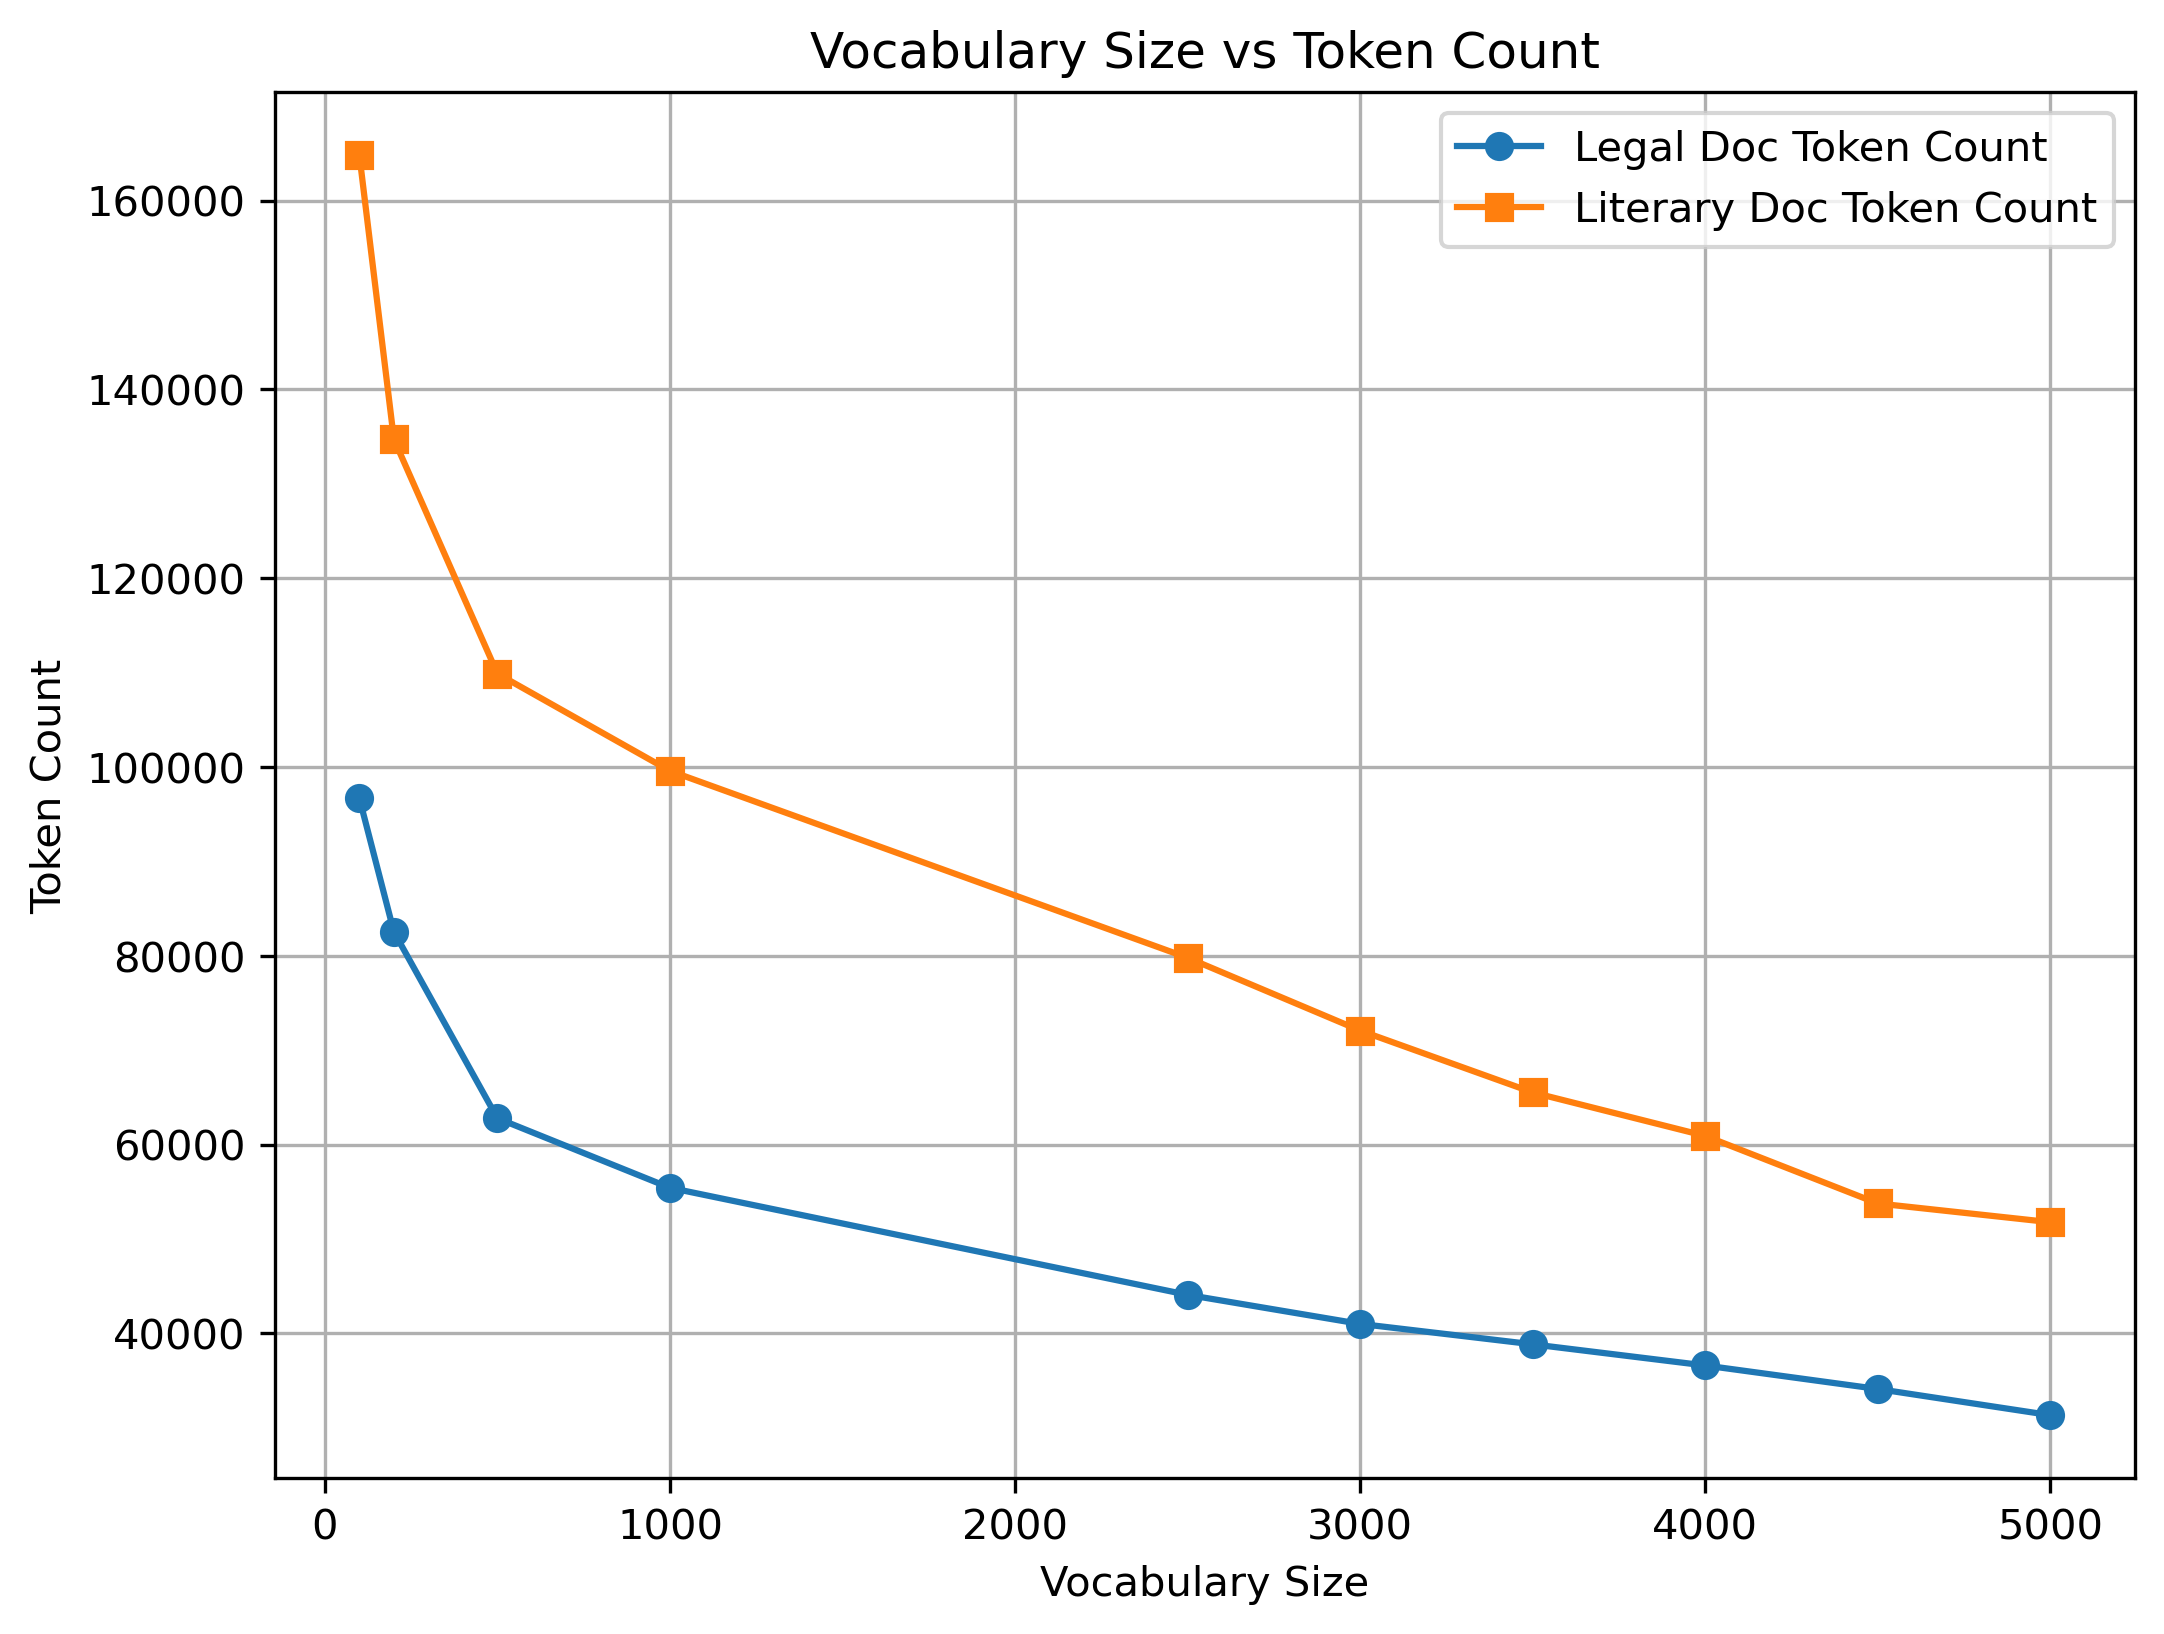
\includegraphics[width=0.6\textwidth]{plot.png}
  \caption{Vocab size vs Token Count}
  \label{fig:sample-png}
\end{figure}
In the resulting plot, token counts generally decreased as the vocabulary size increased, since more merges naturally yield larger subword segments. Through inspection, \texttt{vocab\_size} = 5{,}000 provided a balance: it minimized unnecessary fragmentation of common words and effectively captured domain-specific terms without introducing excessive out-of-vocabulary issues.

\section{Conclusion}
These figures illustrate key distinctions between the legal and literary domains. The higher total token count in the literary text suggests more descriptive or narrative passages, while the legal text, though shorter overall, has a wide range of technical or procedural terms. The common token overlap of 590 demonstrates that both texts rely on some general English subwords (e.g., articles, pronouns, or very frequent word stems). However, each domain's specialized vocabulary is evident in the large number of exclusive tokens, indicating that legal texts rely on statutes, procedures, and jargon, whereas literary texts employ more creative, descriptive, and potentially archaic or whimsical language. This divergence underlines the value of exploring how domain-specific subwords might benefit distinct NLP tasks.
These experiments emphasize how legal and literary texts diverge in their vocabulary distributions. While a limited set of common subwords appeared in both documents, each domain contained a large number of exclusive tokens. Varying the vocabulary size underscored the trade-off between capturing domain-specific terminology and avoiding long token sequences. Ultimately, a vocabulary of 5{,}000 subwords offered a practical middle ground, aligning well with both textual domains and adequately representing the majority of words without fragmenting them excessively.

\end{document}
